\documentclass{beamer}
\usetheme[coloredtitles]{vub} % This will automatically load all fonts (Roboto and TeX Gyre Adventor
               % for titles), and the VUB colors. Also includes the triangle.

% The \usetheme{vub} command accepts many different options:
% - coloredtitles (background of the title on a slide in VUB style)
% - coloredblocks (colours for theorems etc.)
% - showsection (display the current \section on every slide)

% The `dept` option is special, and replaces the VUB logo with a merged
% VUB-department logo.
% Currently supported:
% - dept=etro
% - dept=soft
% - dept=ai
% - dept=brubotics
% - dept=indi
% If you miss a department logo, file an issue at
% https://gitlab.com/rubdos/texlive-vub/issues

% Read the full documentation at
% https://gitlab.com/rubdos/texlive-vub
\usepackage{graphicx}
\graphicspath{ {images/} }
\title{Cloud Computing}
%\subtitle{Your subtitle} % Can be omitted
\author{Gérard Lichtert}

\begin{document}
\frame{\maketitle} % Automatic titlepage with VUB logo.
\begin{frame}{Architecture}
	\begin{figure}
		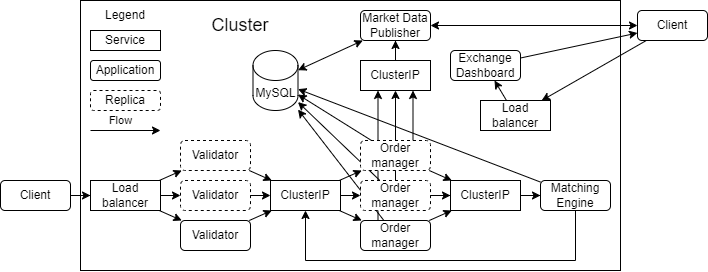
\includegraphics[width=\textwidth]{architecture.drawio.png}
	\end{figure}
\end{frame}
\begin{frame}{Technologies and libraries used}
	\begin{figure}
		
\includegraphics[width=\textwidth]{technologies.drawio.png}
	\end{figure}
\end{frame}
\begin{frame}{Validator}
	\begin{itemize}
		\item Uses fluent-json-schema to pre-validate incoming requests
		\item Forwards validated requests to Order Manager rejects otherwise
	\end{itemize}
\end{frame}
\begin{frame}{Order Manager}
	\begin{itemize}
		\item Uses mysql2/promise to store orders
		\item Forwards orders to Market Data Publisher and Matching Machine
		\item Forwards executions to Market Data Publisher
	\end{itemize}
\end{frame}
\begin{frame}{Matching engine}
	\begin{itemize}
		\item Stores open orders locally
		\item Processes orders using Rxjs
		\item Finds matches
		\item Updates remaining quantity in orders (MySQL)
		\item Sends reduced executions to Order Manager
	\end{itemize}
\end{frame}
\begin{frame}{Market Data Publisher}
	\begin{itemize}
		\item Uses Socket.IO to connect to clients
		\item Uses Rxjs to process orders and executions
		\item Forwards orders and executions to clients subscribed to a symbol
		\item Can read from database to send current data to a client
		\item Computes average price each minute
	\end{itemize}
\end{frame}
\begin{frame}{Exchange Dashboard}
	\begin{itemize}
		\item React application
		\item Uses React's virtual DOM to update UI
		\item Uses a react port of chart.js to display graphs
		\item Uses Socket.IO to subscribe to a symbol and handle events
		\item Can correct local data if it becomes inconsistent
	\end{itemize}
\end{frame}
\begin{frame}{Exchange Dashboard}{Order Book}
	\begin{figure}
		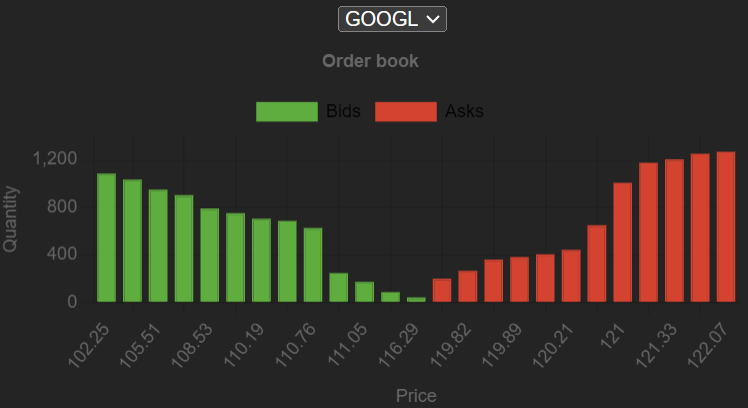
\includegraphics[width=\textwidth]{order-book.png}
	\end{figure}
\end{frame}
\begin{frame}{Exchange Dashboard}{Average price}
	\begin{figure}
		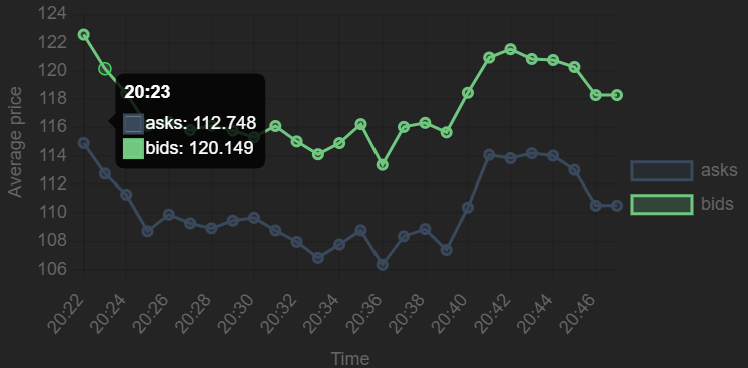
\includegraphics[width=\textwidth]{average-price.png}
	\end{figure}
\end{frame}
\begin{frame}{Demo}
	Timestamps:
	\begin{itemize}
		\item Start descaling 6:40
		\item Actual descaling: 11:10
	\end{itemize}
\end{frame}
\end{document}
